\documentclass{article}
\usepackage{amsmath}
\usepackage{amssymb}
\usepackage{authblk}
\usepackage[font=small,labelfont=bf]{caption}
\usepackage{fullpage}
\usepackage{graphicx}
\usepackage{hyperref}
\usepackage{lineno}
\usepackage{setspace} 
\usepackage{xcolor}
% \usepackage{xeCJK}

\captionsetup{justification=raggedright,singlelinecheck=false}

% Use option lineno for line numbers 
\definecolor{refcolor}{RGB}{245, 5, 189}
\definecolor{lnkcolor}{RGB}{121, 50, 168}
\hypersetup{
    colorlinks=true,
    linkcolor=blue,
    filecolor=magenta,      
    urlcolor=cyan,
    citecolor=refcolor
}

\begin{document}

\bibliographystyle{unsrt}
\linenumbers

\begin{abstract}
Respiratory pathogens such as influenza virus (InfV) and respiratory syncytial 
virus (RSV) are associated with substantial disease burdens among vulnerable 
members of our society and therefore pose significant threats to our healthcare
 system. Infectious diseases caused by these pathogens display strong 
 within-year seasonality - the majority of the disease burden is concentrated 
 in a small number of months. Anecdotally, there may exist some between-year 
 cycles due to factors like genetic drift and immunity waning. When within-year 
 and between-year cycles peak simultaneously, respiratory disease burdens may 
 face significant challenges, which may explain the winter peaks we observed 
 among pediatric outpatient clinics in mainland China in the winter of 2023-24. 
 In this study, we aim to improve our understanding of between-year cycles of 
 infectious diseases caused by InfV and RSV in mainland China.

We looked for data in the published literature that reflect the historical 
variation of disease burden and focus on city-level entities where data exists 
for both InfV and RSV. We started with RSV because the surveillance mechanism 
for this pathogen is relatively newer compared to InfV. We relied on a recently 
published systematic review and identified nine studies that include data we 
are interested in, involving eight cities (i.e. Beijing, Guangzhou, Wuhan, 
Xi'an, Lanzhou, Suzhou, Wenzhou, and Yunfu). We identified further data sources 
on InfV in these cities. Where data is not available, we approximated the 
expected trend using province-level data. 

We used LOESS-based (locally estimated scatterplot smoothing) multiple seasonal 
trend decomposition algorithms (MSTL) to derive within- and between-year cycles. 
We assumed the within-year cycle to be approximately 12 months long and the 
between-year cycle to be longer than 24 months. We optimised for lengths of 
both of these cycles while maximising likelihood and/ or minimising 
autocorrelation coefficients (of the residuals). We discovered variations in 
cycle shapes and lengths by pathogen and location. We are working to project 
the probability of future large winter respiratory epidemics that factor in 
both InfV and RSV infections.

\end{abstract}
\newpage
\doublespacing
\section{Introduction}
Respiratory diseases, notably influenza and Respiratory Syncytial Virus (RSV), significantly impact global health, leading to substantial morbidity and mortality annually. The unpredictability of these diseases' outbreaks underscores the importance of developing accurate prediction models to enhance public health response and preparedness.

The traditional time-series prediction models, primarily focused on single-season cycles, have been instrumental in forecasting the annual patterns of these diseases. However, their efficacy is limited when it comes to capturing the complex interannual variability of disease spread. This variability is influenced by a range of factors beyond simple seasonal trends, making it a critical aspect of disease dynamics that current models often overlook.

This gap in forecasting capabilities points to a need for models that can dynamically adapt to the shifting patterns of disease spread. There is a particular deficiency in models that effectively integrate multiple seasonal patterns and external predictors to accurately forecast interannual fluctuations. This limitation highlights the urgent need for more sophisticated predictive tools.

Our research aims to bridge this gap by exploring the application of the Multiple Seasonal-Trend decomposition using Loess (MSTL) algorithm. MSTL's capacity to model time series with multiple seasonality presents a novel approach to understanding and predicting both annual and interannual disease patterns. This method could significantly improve the accuracy of predictions by providing a more nuanced understanding of disease dynamics.

The potential of improved prediction models like MSTL to offer actionable insights for public health officials is immense. By enabling better planning and resource allocation, these models could play a pivotal role in enhancing public health strategies and intervention planning. Accurately forecasting respiratory disease patterns could, therefore, have broad implications for public health, potentially transforming how outbreaks are managed and mitigated.

This paper is structured as follows: We first delve into the methodology behind employing the MSTL algorithm for capturing interannual cycles. We then present an analysis of the algorithm's efficacy in predicting respiratory disease patterns, followed by a discussion on the implications of our findings for improving disease forecasting and public health strategy. We conclude with reflections on the study's limitations and propose future research directions.


\section{Methods}

\subsection{Analytical Framework }
Figure 1. Framework

\subsection{Data}
We looked for data on the historical disease burden of InfV and RSV at the prefecture/ city level (i.e. administrative level two) for longer than five years with a monthly time scale or finer. Provinces (i.e. administrative level one) in China often cover large geographic areas (e.g. the size of Guangxi alone is comparable to the UK), include multiple climate zones, and have drastically different socioeconomic statuses internally - conducting analysis on the province level may mask distinctive experiences in terms of respiratory infectious diseases. In order to identify cities with data on both InfV and RSV, we started with RSV, which has newer and less consistent surveillance systems compared to InfV in the context of mainland China. We relied on a recently published systematic review on the within-year seasonality of RSV \cite{guo2024respiratory} and found nine studies that met our inclusion criteria, covering eight cities: Beijing, Lanzhou, Suzhou, Guangzhou, Wenzhou, Xi'an, Yunfu, and Wuhan (\hyperref[fig_1]{Figure 1}). For RSV, the metric for all studies used were \textbf{BLAH}.

With these cities in mind, we searched for data on InfV using the same inclusion criteria. We searched in PubMed was structured as follows: “(Influenza, Human [MeSH Terms] OR influenza [Title/Abstract]) AND (China [MeSH Terms] OR China [Title/Abstract] OR Chinese [Title/Abstract]) AND "last 10 years"[PDat]”. We identified existing literature for each city. The outcome variable include \textbf{blah blah and blah}. In order to make a comparison between cities and pathogens, we did the \textbf{blah normalisation}.

\begin{figure}[htbp]
  \centering
  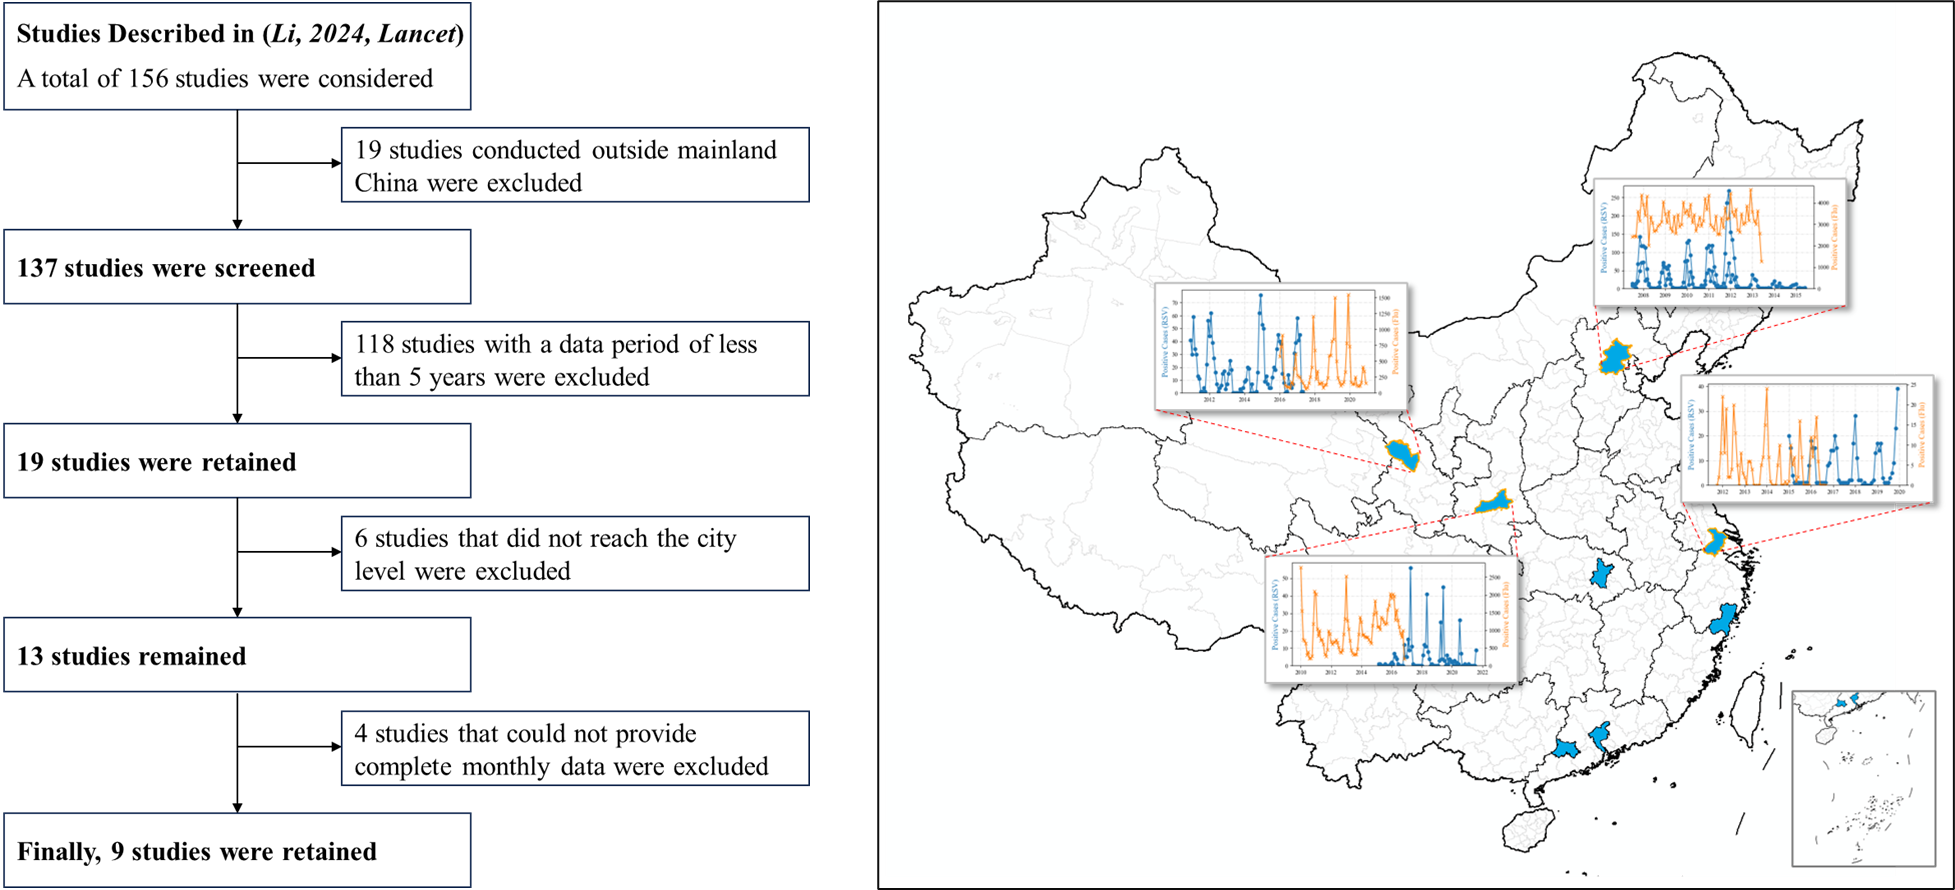
\includegraphics[width=0.8\textwidth]{Flu-RSV.png}
  \caption{Selection and Compilation of Influenza and RSV Data. (a) Data Selection Process; (b) Geographical Scope and Data Representation for Influenza and RSV.}
  \label{fig_1_bak}
\end{figure}

\subsection{Deriving the within- and between-year cycles}
We used a smoothing-based algorithm to derive the within- and between-year cycles in the disease burden of InfV and RSV. The essence of this algorithm is LOESS (Locally Estimated Scatterplot Smoothing). Seasonal-Trend decomposition using LOESS (STL) is commonly used to derive within-year cycles in time-series data, assuming single internal cycles (e.g. 12 months- or 52 weeks-long). The smoothing-based approach is numerically more flexible compared to other approaches that require researchers to make assumptions about expected mathematical forms (e.g. cosiner models or cubic spline-based models) \cite{madaniyazi2022assessing}.  

In this study, we used MSTL (Multiple Seasonal-Trend decomposition using LOESS), which allows for more than one internal cycle. We assumed the within-year cycle lengths to be between $X_1$ and $X_2$ and between-year cycle lengths to be between 18 and 36 months. The upper limit of the between-year cycle lengths is constrained by the total lengths of the series. We looked for the most appropriate sets of within- and between-year cycle lengths through grid-search, by maximising likelihoods and by minimising auto-correlation coefficients among residuals. At the end of this analytical pipeline, we would have a pair of within- and between-year cycles for each city and each pathogen. 

The uncertainty around the within- and between-year cycles derived are assessed \textbf{XXXXXX}. The differences in terms of between-year cycle lengths were compared using KL divergence.


\newpage


\newpage







\subsection{Projecting Disease Burden for Multiple Pathogens }


\section{Results}
\begin{itemize}
    \item Exhibit 1. Revised Figure 1, map in the middle, figures on the two sides
    \begin{figure}[htbp]
      \centering
      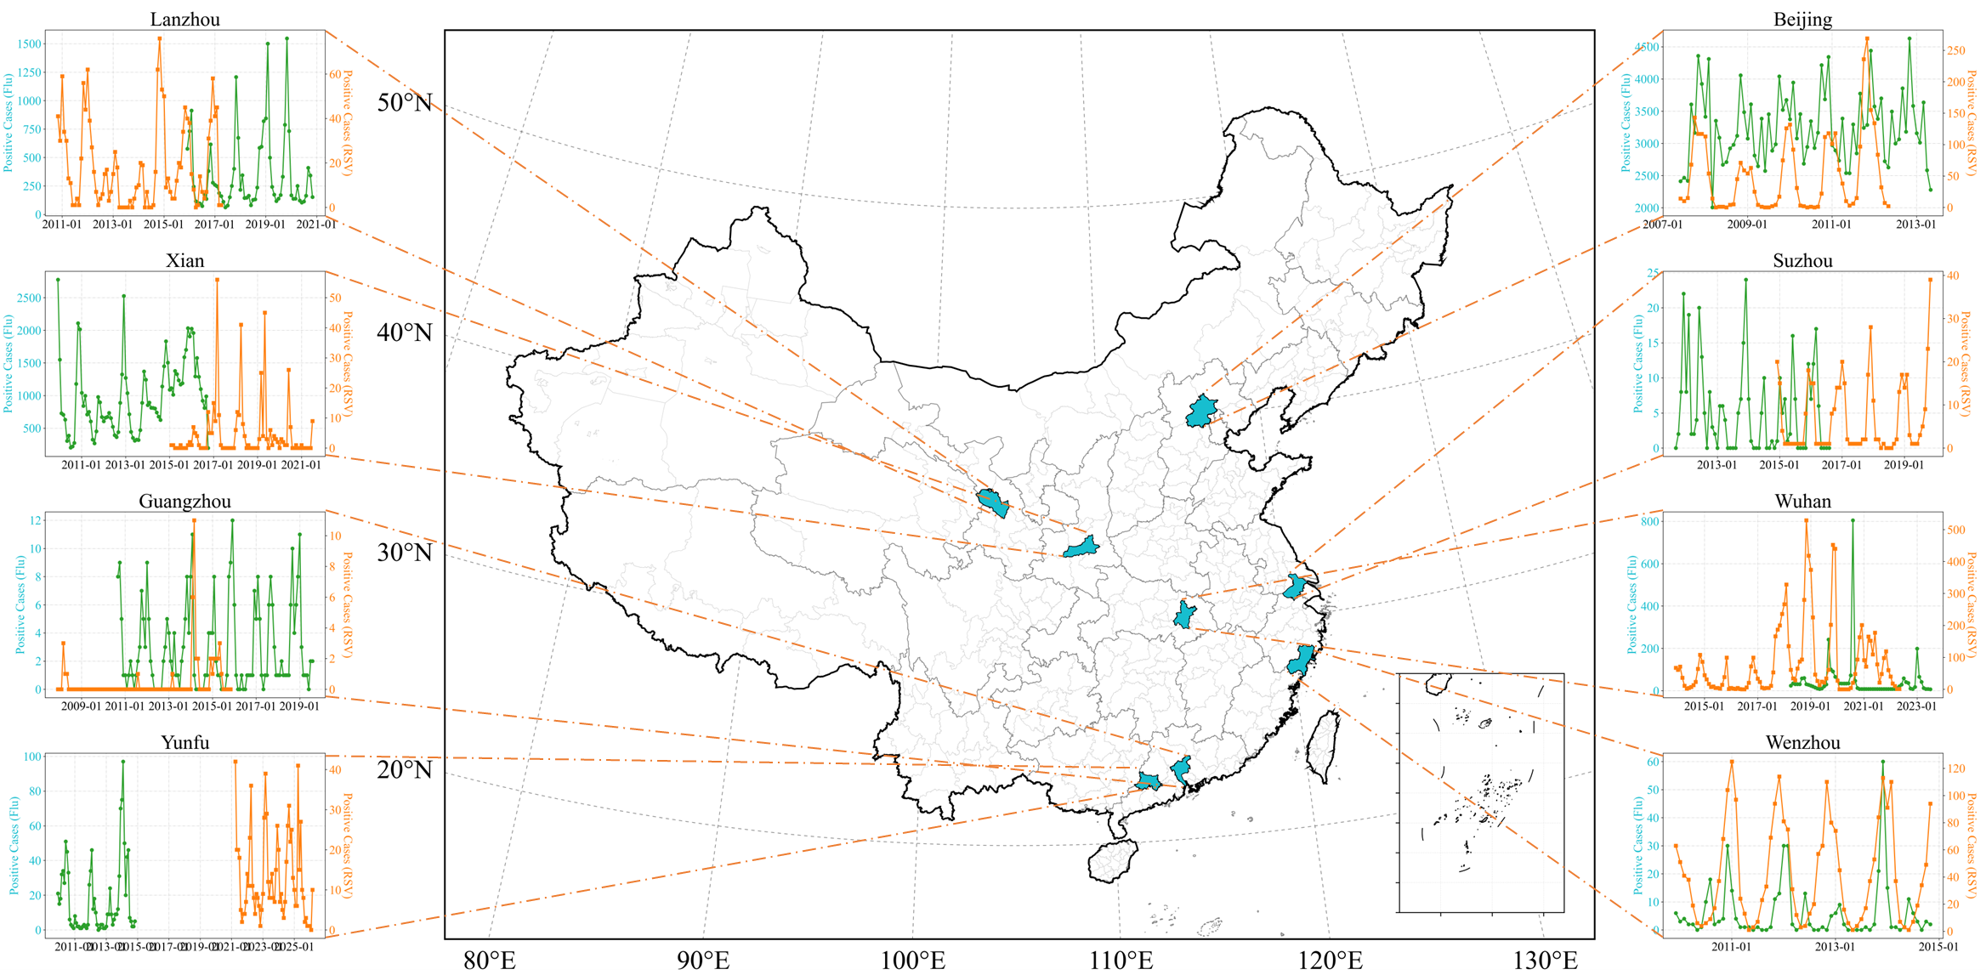
\includegraphics[width=1.0\textwidth]{figs/Figure 1.png}
      \caption{Dataset}
      \label{fig_1}
    \end{figure}    


    
    \item Exhibit 2. Visualisations of cycles
    \begin{figure}[htbp]
      \centering
      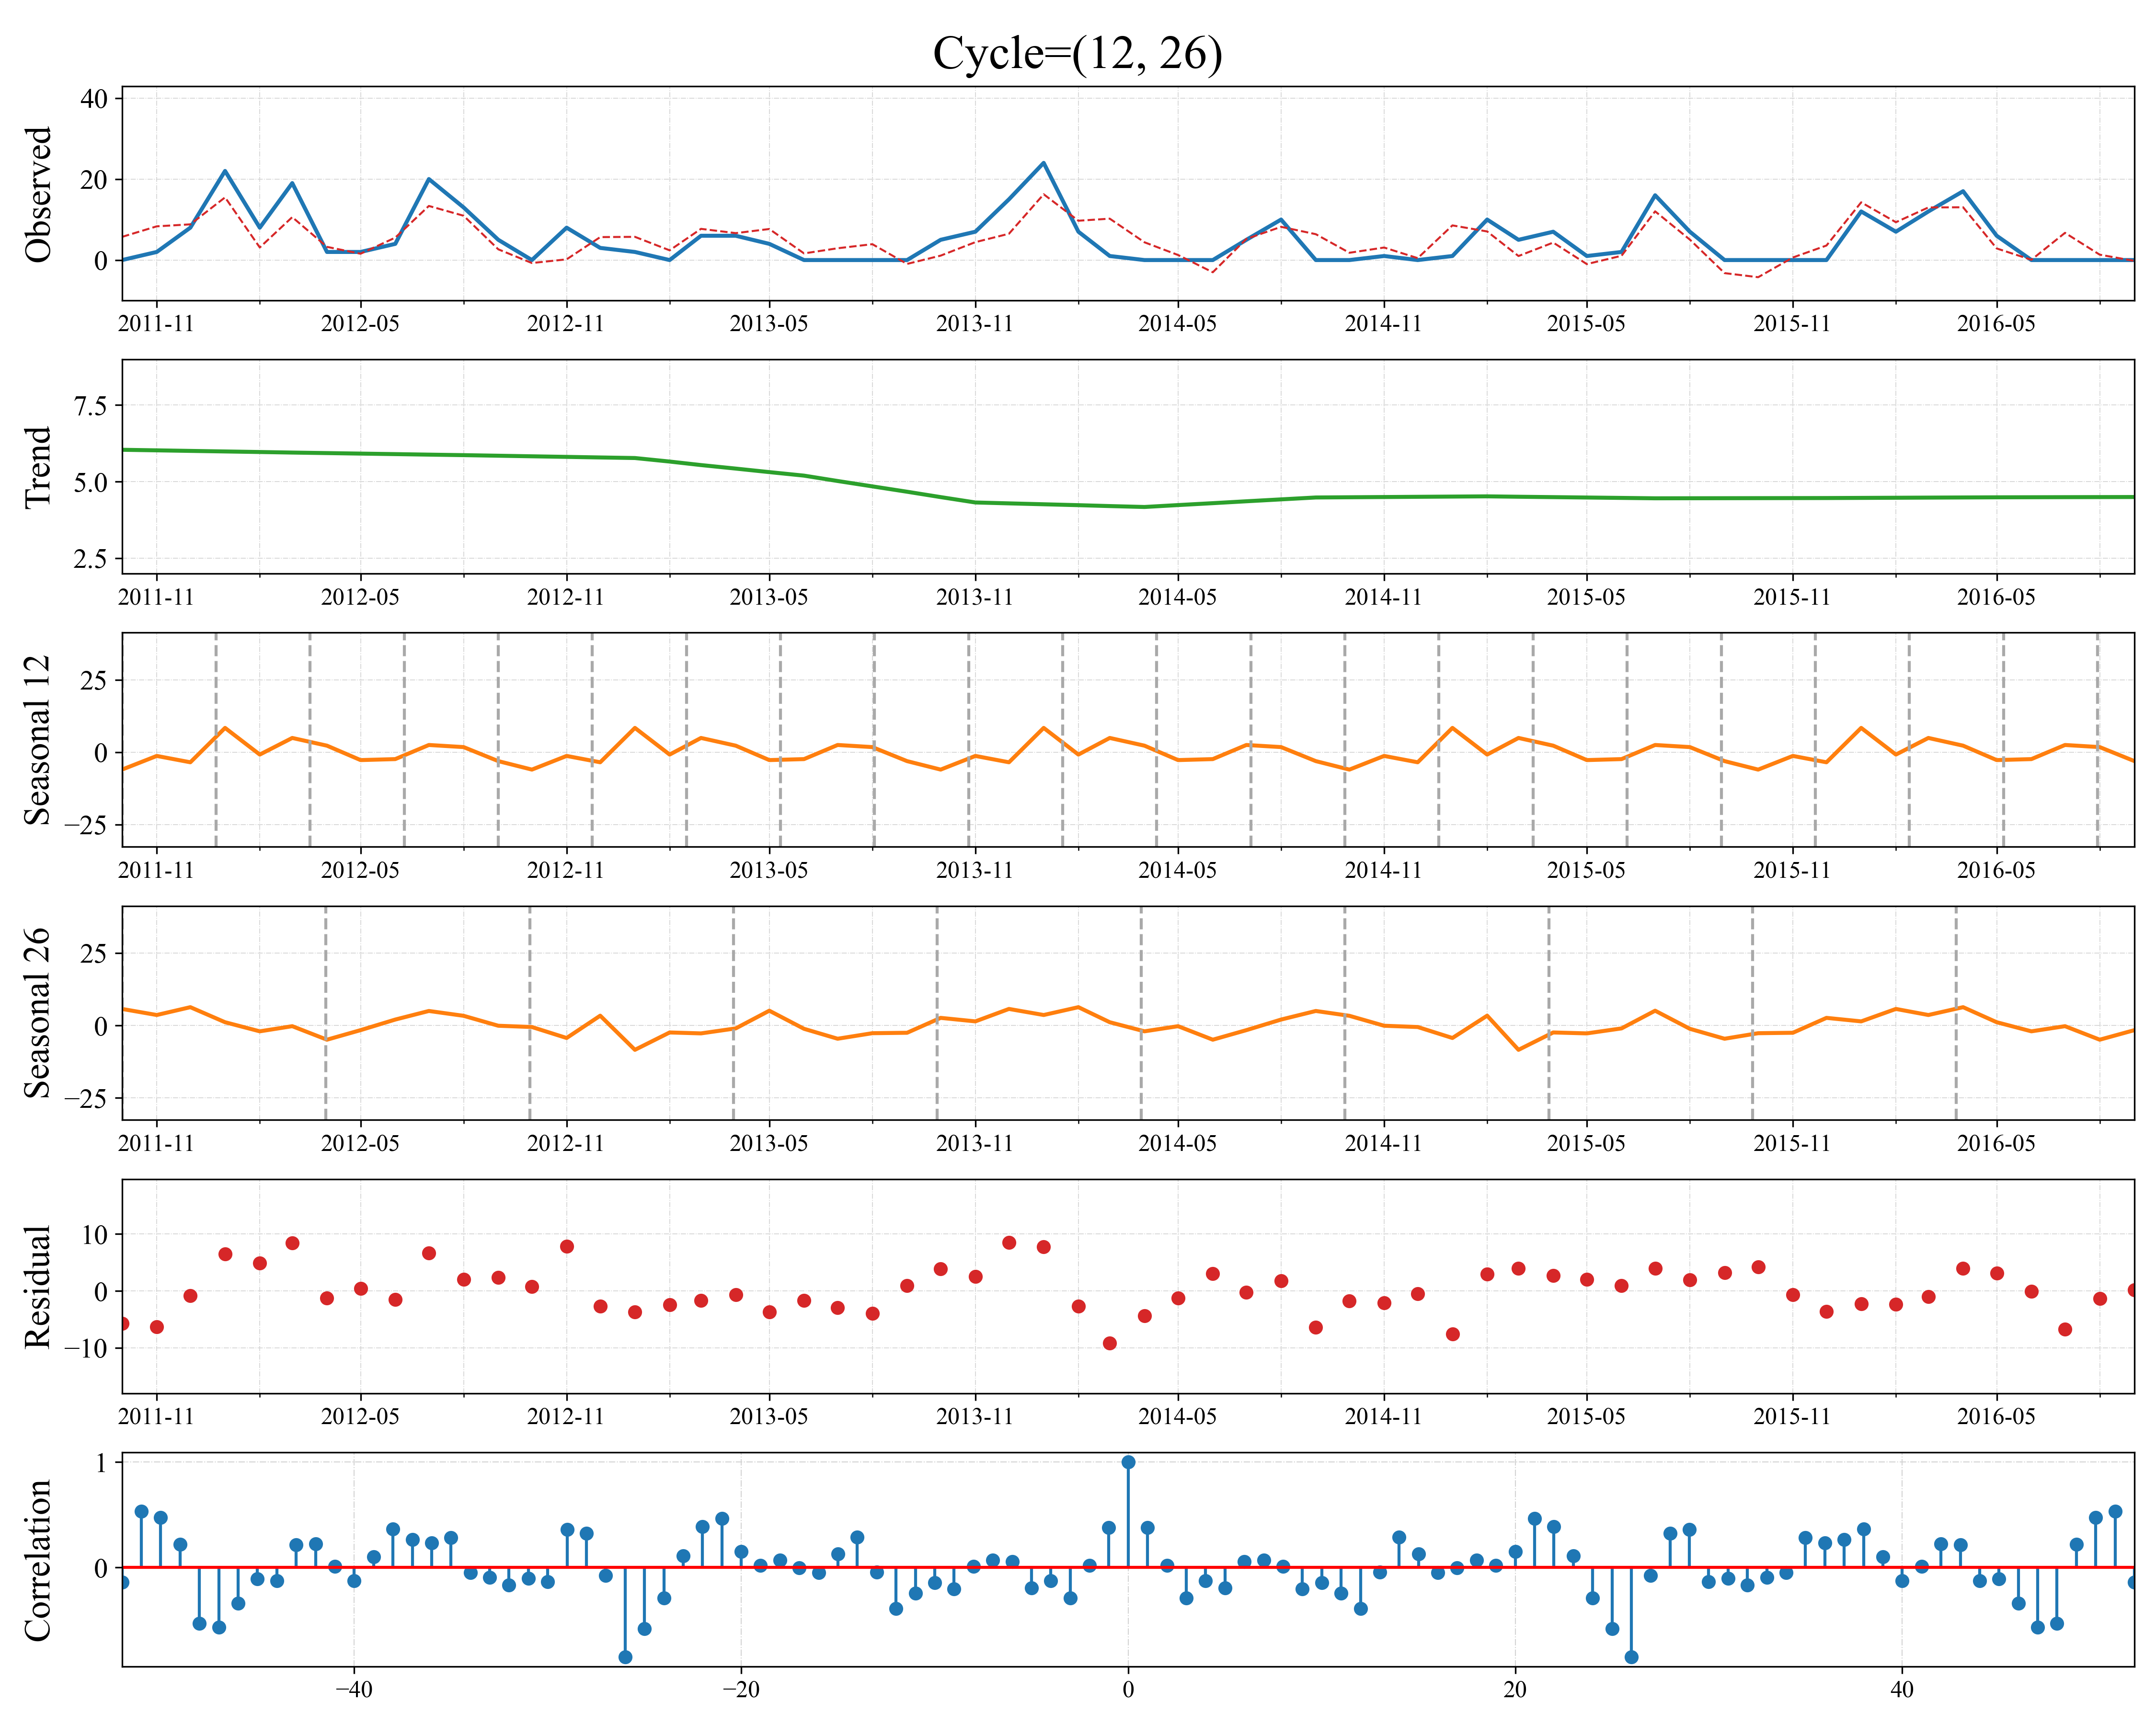
\includegraphics[width=1.0\textwidth]{figs/decomposition_cycle_12_26.png}
      \caption{Decomposition}
      \label{fig_2}
    \end{figure}    
    
    \item Exhibit 3. Statistical features of cycles derived:  shapes, duration, peaks-to-trough ratios, peak timing
        \begin{itemize}
            \item comparison to single cycle algorithm
        \end{itemize}

    \begin{figure}[htbp]
      \centering
      \includegraphics[width=1.0\textwidth]{figs/projections_selected_cycles.png}
      \caption{Projections}
      \label{fig_3_1}
    \end{figure}    
    
    \begin{figure}[htbp]
      \centering
      \includegraphics[width=1.0\textwidth]{figs/projections_confidence_interval.png}
      \caption{Projections-CI}
      \label{fig_3_2}
    \end{figure}    

    

        
    \item Exhibit 4. Projection, risks of multi-epidemics
    \item Exhibit 5. Spatial heterogeneity by city
\end{itemize}

\bibliography{references}
\end{document}






